\subsection{Convergence of the posterior distribution}

We wish to study the convergence of the posterior distribution obtained using the probabilistic method with respect to the true posterior distribution. In the following, we consider only the distance between the target distributions given by an exact algorithm and the target distribution of the MCMC with approximated likelihood, disregarding the error due to the MCMC approximation. This assumption is rather strong, as the convergence of MCMC can be slow depending on the initial condition, the prior distribution and the proposal distribution. \\
In order to study the convergence, it is necessary to introduce a notion of distance between two probability measures. A standard measure is the \textit{total variation distance}, defined in the following.
\begin{definition} Given two probability measures $\nu$ and $\mu$ on a measurable space $(\mathcal{X}, \mathcal{B}(\mathcal{X}))$, the total variation distance between $\nu$ and $\mu$ is defined as
\begin{equation}
	d_{\mathrm{TV}}(\nu,\mu) \defeq \sup_{A\in \mathcal{B}(\mathcal{X})} \left|\nu(A) - \mu(A)\right|.
\end{equation}
Moreover, if $\nu$ and $\mu$ admit a densities $f$ and $g$ respectively with respect to a dominating measure $\lambda$, then the total variation distance can be expressed as
\begin{equation}
	d_{\mathrm{TV}}(\nu,\mu) \defeq \frac{1}{2} \int_{\mathcal{X}} (f(x) - g(x))\dd \lambda(x).
\end{equation}
\end{definition}
\noindent Other notions of distance can be employed when the total variation distance is not practical to compute, such as the Hellinger distance, which is defined as follows \cite{GiS02}.
\begin{definition} If $f, g$ are densities of the measures $\mu$ and $\nu$ on $(\R^n, \mathcal{B}(\R^n))$ with respect to the Lebesgue measure, the Hellinger distance between $\nu$ and $\mu$ is defined as
\begin{equation}
	\Hell^2(\mu, \nu) \defeq \frac{1}{2}\int_{\R^n}\left(\sqrt{f(x)} - \sqrt{g(x)}\right)^2\dd x
\end{equation}
\end{definition}
\noindent The Hellinger distance allows us to estimate the total variation distance as the following inequalities hold \cite{GiS02}
\begin{equation}\label{eq:TVvsHell}
	\frac{\Hell^2(\mu, \nu)}{2} \leq d_{\mathrm{TV}}(\mu, \nu) \leq \Hell(\mu, \nu).
\end{equation}
Let us consider the posterior distribution given by MCMC with approximated likelihood. We can compute the second moment of the Hellinger distance as
\begin{equation}
\begin{aligned}
2\E^\xi\left[\Hell^2(\pi(\theta|\mathcal{Y}),\pi^M_h(\theta|\mathcal{Y}))\right] &= \E^\xi\left[\int \left(\sqrt{\pi(\theta|\mathcal{Y})} - \sqrt{\pi^M_h(\theta|\mathcal{Y})}\right)^2 \dd \theta\right] \\
&= \E^\xi\left[\int \left(\sqrt{\prior(\theta) \diffL(\mathcal{Y}|\theta)} - \sqrt{\prior(\theta) \diffL^M_h(\mathcal{Y}|\theta)}\right)^2 \dd \theta \right]\\
&= \int \E^\xi\left[\left(\sqrt{\diffL(\mathcal{Y}|\theta)} - \sqrt{\diffL^M_h(\mathcal{Y}|\theta)}\right)^2\right] \dd \prior(\theta)  \\
&= \int \MSE\left(\sqrt{\diffL^M_h(\mathcal Y|\theta)}\right) \dd \prior(\theta) \\
&\leq \int C(\theta)h^{2q} \dd \prior(\theta) \\
&= h^{2q} \int C(\theta) \dd \prior(\theta),
\end{aligned}
\end{equation}
where $C(\theta)$ is the constant appearing in Proposition \ref{prop:MSE}. Let us remark that the constant depends on the Lipschitz constant of the function defining the ODE, which depends non-trivially on $\theta$. Finally, defining 
\begin{equation}
	\tilde C \defeq \sqrt{\frac{1}{2} \int C(\theta) \dd \prior(\theta)}, 
\end{equation}
we get the following bound on the second moment of the Hellinger distance between the approximated posterior and the posterior obtained with the exact solution 
\begin{equation}
	\E^\xi\left[\Hell^2(\pi(\theta|\mathcal{Y}),\pi^M_h(\theta|\mathcal{Y}))\right] \leq \tilde C^2 h^{2q}.
\end{equation}
Then, thanks to Jensen's inequality
\begin{equation}
\begin{aligned}
	\E^\xi\left[\Hell(\pi(\theta|\mathcal{Y}),\pi^M_h(\theta|\mathcal{Y}))\right] &\leq \E^\xi\left[\Hell^2(\pi(\theta|\mathcal{Y}),\pi^M_h(\theta|\mathcal{Y}))\right]^{1/2} \\
	&\leq \tilde C h^q.
\end{aligned}
\end{equation}
Let us remark that thanks to \eqref{eq:TVvsHell}, this bound is equally true for the total variation distance. 

\subsection{Convergence of the parameter mean}\label{sec:ParH}
We are now interested in the convergence of the expectation of the parameter $\theta$ inferred by MCMC. Let us consider a function $g \colon \R^{N_p} \to \R$ such that $g \in L^\infty(\R^{N_p})$. Then, we wish to bound the distance between the expectation of $g(\theta)$ computed with respect to the true measure and to the measure targeted by MCMC implemented with the probabilistc solver and time step $h$. Thanks to the previous result on the total variation distance we get
\begin{equation}
\begin{aligned}
	\E^\xi\abs{\E^\pi\left[g(\theta)\right] - \E^{\pi_h^M}\left[g(\theta)\right]} &= \E^\xi\abs{\int g(\theta)(\pi(\theta|\mathcal{Y}) - \pi_h^M(\theta|\mathcal{Y}))\dd \theta}\\
	&\leq \norm{g}_\infty \E^\xi \left[\int \abs{\pi(\theta|\mathcal{Y}) - \pi_h^M(\theta|\mathcal{Y})} \dd \theta\right] \\
	&= 2 \norm{g}_\infty \E^\xi\left[d_{\mathrm{TV}}(\pi, \pi_h^M)\right] \\
	&\leq 2 \norm{g}_\infty C h^{q}.
\end{aligned}
\end{equation}
We can now compute the variance of the expectation of $g(\theta)$ computed MCMC and the probabilistic integrator as
\begin{equation}
\begin{aligned}
	\Var^\xi (\E^{\pi_h^M}\left[g(\theta)\right]) &= \Var^\xi \left(\int g(\theta) \pi^M_h (\theta) \dd \theta \right) \\
	&= \Var^\xi \left(\int g(\theta) \diffL^M_h (\mathcal{Y}|\theta) \dd \prior(\theta) \right) \\
	&= \int g(\theta) \Var^\xi(\diffL^M_h (\mathcal{Y}|\theta)) \dd \prior(\theta) \\
	&\leq Ch^{2q} \int g(\theta) \dd \prior(\theta) \\
	&= \hat C h^{2q},
\end{aligned}
\end{equation}
where we applied Proposition \ref{prop:MSE}. Hence, the MSE of this estimation is bounded quadratically with respect to the order of the employed Runge-Kutta method, i.e.,  
\begin{equation}
\begin{aligned}
	\MSE(\E^{\pi_h^M}\left[g(\theta)\right]) &= \E^\xi\left[\E^{\pi_h^M}\left[g(\theta)\right] - \E^{\pi}\left[g(\theta)\right]\right]^2 + \Var^\xi(\E^{\pi_h^M}\left[g(\theta)\right]) \\
	&\leq C h^{2q}.
\end{aligned}
\end{equation}

\subsection{Considerations on the MCMC approximation}

All the results of convergence presented above regard the approximation of the true posterior distribution with the posterior distribution approximated with time step $h$. These estimations are true if we have access to these distributions. In practice, if the posterior distribution is $\pi(\cdot)$, we use a MCMC method to get the Monte Carlo approximation
\begin{equation}
	\E^\pi[g(\theta)] \approx \frac{1}{N} \sum_{i = 1}^{N} g(\theta^{(i)}),
\end{equation}
where $\theta^{(i)}$, $i = 1, \ldots, N$, are the samples given by MCMC. Let us denote by $\hat g(\theta)$ the Monte Carlo estimator, i.e.,
\begin{equation}
	\hat g(\theta) = \frac{1}{N} \sum_{i = 1}^{N} g(\theta^{(i)}).
\end{equation} 
It is meaningful to study the relation between $\hat g(\theta)$ and $\E^\pi[g(\theta)]$ with respect to the number of samples $N$. The main issue is given by the Markov chain property of the samples. In standard Monte Carlo, the samples are independent and therefore estimating its mean and variance is straightforward, as well as studying the asymptotic properties with the central limit theorem. A central limit theorem is available for Markov chains under regularity assumptions on the Markov kernel \cite{Jon04}, i.e., with the notation introduced above
\begin{equation}\label{eq:CLTMarkov}
	\sqrt{N}(\hat g(\theta) - \E^\pi[g(\theta)]) \totext{d} \mathcal{N}(0, \sigma^2_g),
\end{equation}
where the convergence is in the distributional sense and we can define the variance of the Monte Carlo estimator as
\begin{equation}
\sigma^2_g \defeq \Var^\pi(g(\theta^{(0)})) + 2\sum_{i = 1}^{\infty} \mathrm{Cov}^\pi(g(\theta^{(0)}), g(\theta^{(i)})) < \infty.
\end{equation}
In general, it is not possible to compute analytically $\sigma_g$, but many techniques have been proposed in order to estimate it from the Markov chain itself. A common method \cite{FlJ10} is to compute the \textit{batch means} of the Markov chain and use them to estimate $\sigma^2_g$. \\
Let us suppose that there exist two integers $a_N, b_N$ such that $N = a_Nb_N$. Then we define the following $a_N$ non-overlapping means of subsequences contained in the Markov chain of length $b_N$
\begin{equation}
	\bar g_k(\theta) = \frac{1}{b_N} \sum_{i=1}^{b_N} g(\theta^{(kb_N + i)}), \quad k = 0, \ldots, a_N - 1. 
\end{equation} 
Finally, we can build an estimator of $\sigma_g^2$ computing the population variance of the $\bar g_k$ with respect to $\hat g$, i.e.,
\begin{equation}
	\hat\sigma^2_{\mathrm{BM}} = \frac{b_N}{a_N - 1} \sum_{k=0}^{a_N -1}(\bar g_k - \hat g)^2. 
\end{equation}
Under regularity conditions on the posterior distribution $\pi$ and the transition kernel $P$ defining the Markov chain, and if $a_N$ and $b_N$ are growing functions of $N$ such that $a_N \to \infty$, $b_N \to \infty$ if $N \to \infty$, with $b_N / N \to 0$, it is possible to show \cite{FlJ10} that this estimator is \textit{mean-square consistent}, i.e.,
\begin{equation}
	\MSE(\hat\sigma^2_{\mathrm{BM}}) \totext{N\to\infty} 0.
\end{equation}
In \cite{FlJ10}, the authors suggest to choose $b_N$ to be the square or cubic root of $N$ for accelerating the convergence of the MSE to zero, i.e.,
\begin{equation}
	b_N = \floor{N^{1/3}}, \quad \text{or,} \quad b_N = \floor{N^{1/2}}.
\end{equation}
We can deduce from the limit in \eqref{eq:CLTMarkov} that the standard deviation of the MCMC estimator decreases asymptotically linearly with respect to $N^{1/2}$. Therefore, in order to observe the convergence rates with respect to $h$ presented in Section \ref{sec:ParH}, the number of samples of the drawn in the MCMC algorithm will have to be considerably high.

\subsubsection{Numerical experiment - Batch means estimator}

In this experiment we wish to verify numerically the validity of the batch mean estimator presented above. Therefore, we consider the FitzHug-Nagumo model \eqref{eq:FitzNag} with ten observations $\mathcal{Y}$ equispaced in the time span $0 \leq t \leq 10$. We run MCMC algorithms with approximated likelihood with $h = 0.1$ and growing number of iterations $N = \{1000, 2000, 4000, 8000, 16000, 32000, 64000\}$, and equal starting points. For each value of $N$, we perform $400$ repetitions of the Markov chain and compute the population variance of the estimator $\hat g(\theta)$ as a function of $N$ in order to obtain an estimation of $\sigma^2_g$, where the function $g$ we consider in this experiment is $g(\theta) = \theta^T\theta$. We then compute the batch mean estimator $\hat \sigma_{\mathrm{BM}}$ using $b = \floor{N^{1/2}}$ for each repetition and average the results in order to obtain a function of the number of samples $N$. Results (Figure \ref{fig:BatchMeans}) show that the variance $\sigma^2_g$ converges as predicted linearly with $N$. Moreover, the estimation provided by $\hat \sigma_{\mathrm{BM}}$ is coherent with the theoretical results. We remark that the batch mean estimator seems to converge to the true value of the sample variance with a quadratic order with respect to the number of samples. Further theoretical and literature investigations will be necessary to study this behavior. Hence, we can conclude that the batch means method provides a consistent estimation of the variance, without running several repetitions of the chains to verify their variance.

\begin{figure}[t]
	\centering
	\begin{subfigure}{0.49\linewidth}
		\centering
		\resizebox{1.0\linewidth}{!}{% This file was created by matlab2tikz.
%
%The latest EFupdates can be retrieved from
%  http://www.mathworks.com/matlabcentral/fileexchange/22022-matlab2tikz-matlab2tikz
%where you can also make suggestions and rate matlab2tikz.
%
\definecolor{mycolor1}{rgb}{0.00000,0.44700,0.74100}%
\definecolor{mycolor2}{rgb}{0.85000,0.32500,0.09800}%
%
\begin{tikzpicture}

\begin{axis}[%
width=4.717in,
height=3.721in,
at={(0.791in,0.502in)},
scale only axis,
xmode=log,
xmin=1000,
xmax=100000,
xminorticks=true,
xlabel={$N$},
xlabel style = {font=\LARGE},
ymode=log,
ymin=1e-05,
ymax=0.01,
yminorticks=true,
ymajorgrids,
xmajorgrids,
mark size = 3,
axis background/.style={fill=white},
legend style={legend cell align=left,align=left,draw=white!15!black},
ticklabel style={font=\LARGE},legend style={font=\LARGE},title style={font=\LARGE}
]
\addplot [color=mycolor1,solid,mark=o,mark options={solid}]
  table[row sep=crcr]{%
1000	0.00319872069944162\\
2000	0.0015198533552747\\
4000	0.000861085186590669\\
8000	0.000351717575842792\\
16000	0.000167008594366653\\
32000	7.63488996761454e-05\\
64000	3.71915765755024e-05\\
};
\addlegendentry{$\Var^\pi(\hat g(\theta))$};

\addplot [color=mycolor2,solid,mark=asterisk,mark options={solid}]
  table[row sep=crcr]{%
1000	0.00205474165782296\\
2000	0.00121491896622609\\
4000	0.000640684648553251\\
8000	0.000331430067672156\\
16000	0.00016174899548401\\
32000	7.69800956282351e-05\\
64000	3.69556790826172e-05\\
};
\addlegendentry{$\hat \sigma^2_{\mathrm{BM}}/N$};

\addplot [color=black,dashed]
  table[row sep=crcr]
	\end{subfigure}
	\begin{subfigure}{0.49\linewidth}
		\centering
		\resizebox{1.0\linewidth}{!}{% This file was created by matlab2tikz.
%
%The latest EFupdates can be retrieved from
%  http://www.mathworks.com/matlabcentral/fileexchange/22022-matlab2tikz-matlab2tikz
%where you can also make suggestions and rate matlab2tikz.
%
\definecolor{mycolor1}{rgb}{0.00000,0.44700,0.74100}%
%
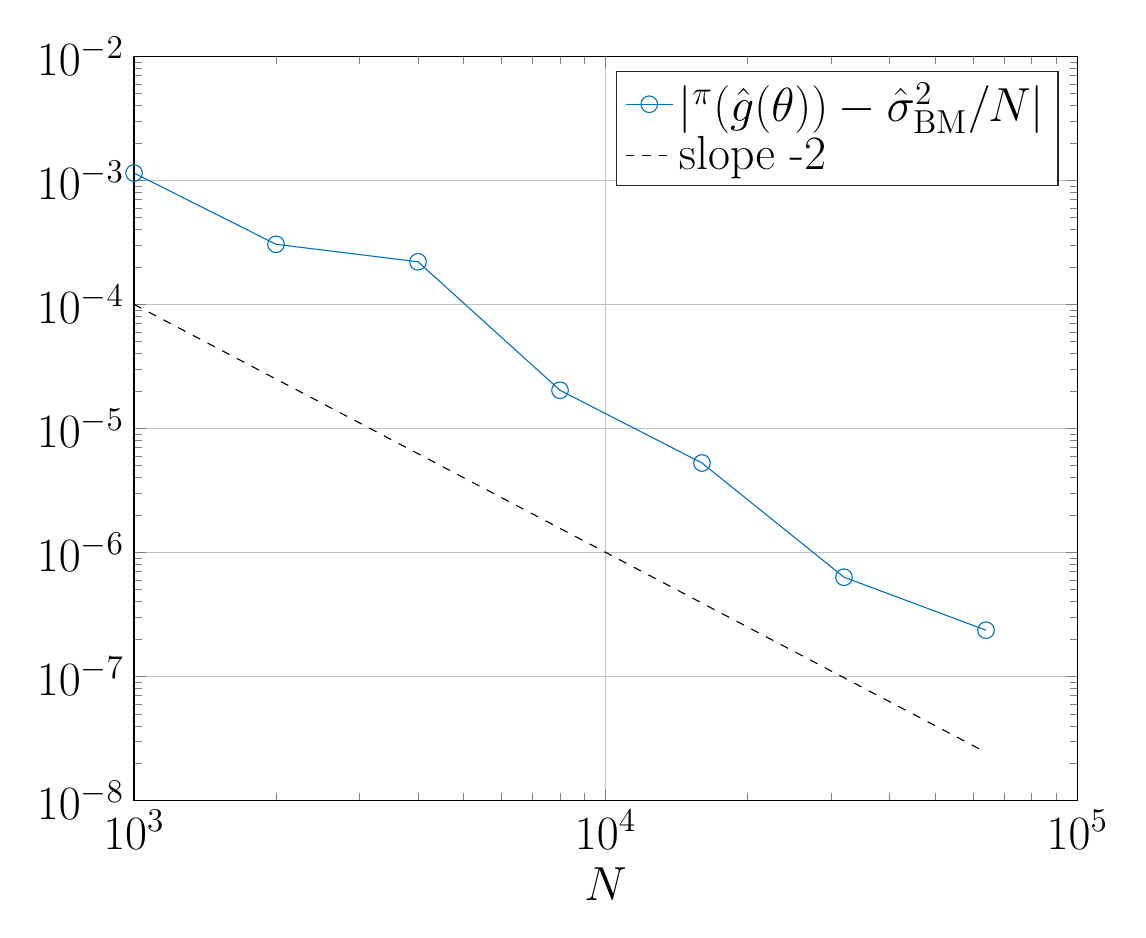
\begin{tikzpicture}

\begin{axis}[%
width=4.717in,
height=3.721in,
at={(0.791in,0.502in)},
scale only axis,
xmode=log,
xmin=1000,
xmax=100000,
xminorticks=true,
xlabel={$N$},
xlabel style = {font=\LARGE},
ymode=log,
ymin=1e-08,
ymax=0.01,
yminorticks=true,
ymajorgrids,
xmajorgrids,
mark size = 3,
axis background/.style={fill=white},
legend style={legend cell align=left,align=left,draw=white!15!black},
ticklabel style={font=\LARGE},legend style={font=\LARGE},title style={font=\LARGE}
]
\addplot [color=mycolor1,solid,mark=o,mark options={solid}]
  table[row sep=crcr]{%
1000	0.00114397904161866\\
2000	0.000304934389048606\\
4000	0.000220400538037418\\
8000	2.02875081706361e-05\\
16000	5.25959888264269e-06\\
32000	6.31195952089693e-07\\
64000	2.35897492885213e-07\\
};
\addlegendentry{$|\Var^\pi(\hat g(\theta)) - \hat \sigma^2_{\mathrm{BM}}/N|$};

\addplot [color=black,dashed]
  table[row sep=crcr]
	\end{subfigure}
	\caption{Variance of the Monte Carlo approximation given by MCMC with respect to the number of samples $N$. The convergence to zero is linear with respect to the number of samples. The estimator given by the batch means method converges to the true value of the variance with a quadratic order.}
	\label{fig:BatchMeans}
\end{figure}

\subsection{Numerical experiment - Convergence of the posterior distribution}

We consider the FitzHug-Nagumo model \eqref{eq:FitzNag} and produce observations $\mathcal{Y}$ at times $t_i = i$ for $i = 1, \ldots, 10$ from a reference solution with additive noise with variance $10^{-2}$. We produce a reference posterior distribution using the result of a MCMC algorithm obtained with a small time step $h$. We then vary $h$ in order to observe the convergence of the posterior distribution towards the reference, as well as the convergence of the Monte Carlo estimation. We consider $100000$ iterations of RAM applied to MCWM. As discussed above, the number of trajectories $M$ used to approximate the numerical likelihood does not have an influence on the convergence rate of the posterior distribution to the true posterior. Therefore, we just fix $M$ to be equal to one. We consider as the function $g$ of the parameter the Euclidean norm, therefore we consider the approximation
\begin{equation}
	\norm{\theta} \approx 10^{-6} \sum_{i = 1}^{10^6} \norm{\theta^{(i)}}.
\end{equation}
Results	(Figure \ref{fig:ConvergenceMCMC}) show the convergence obtained averaging 10 realizations of the entire MCMC chain used in order to simulate the expectation with respect to the random variable $\sigma$.

\begin{figure}[t]
	\centering
	\begin{subfigure}{0.49\linewidth}
		\centering
		\resizebox{1.0\linewidth}{!}{% This file was created by matlab2tikz.
%
%The latest EFupdates can be retrieved from
%  http://www.mathworks.com/matlabcentral/fileexchange/22022-matlab2tikz-matlab2tikz
%where you can also make suggestions and rate matlab2tikz.
%
\definecolor{mycolor1}{rgb}{0.00000,0.44700,0.74100}%
%
\begin{tikzpicture}

\begin{axis}[%
width=4.717in,
height=3.721in,
at={(0.791in,0.502in)},
scale only axis,
xmode=log,
xmin=0.001,
xmax=0.1,
xminorticks=true,
ymode=log,
ymin=0.001,
ymax=1,
yminorticks=true,
mark size = 3,
xmajorgrids,
ymajorgrids,
xlabel = {$h$},
xlabel style = {font = \LARGE},
axis background/.style={fill=white},
legend style={at={(0.97,0.03)},anchor=south east,legend cell align=left,align=left,draw=white!15!black},
ticklabel style={font=\LARGE},legend style={font=\LARGE},title style={font=\LARGE}
]
\addplot [color=mycolor1,solid,mark=o,mark options={solid}]
  table[row sep=crcr]{%
0.04	0.1123258357954\\
0.02857	0.0727138687866972\\
0.0204	0.0481898817135708\\
0.0147	0.0315365035547742\\
0.01052	0.0205454707551366\\
0.00751	0.0140770405527581\\
0.00537	0.00899400013529372\\
0.00384	0.00595686479536912\\
0.00274	0.0037036370712952\\
};
\addlegendentry{$|\|\hat \theta\| - \|\theta\| |$};

\addplot [color=black,dashed]
  table[row sep=crcr]
	\end{subfigure}
	\begin{subfigure}{0.49\linewidth}
		\centering
		\resizebox{1.0\linewidth}{!}{% This file was created by matlab2tikz.
%
%The latest EFupdates can be retrieved from
%  http://www.mathworks.com/matlabcentral/fileexchange/22022-matlab2tikz-matlab2tikz
%where you can also make suggestions and rate matlab2tikz.
%
\definecolor{mycolor1}{rgb}{0.00000,0.44700,0.74100}%
%
\begin{tikzpicture}

\begin{axis}[%
width=4.717in,
height=3.721in,
at={(0.791in,0.502in)},
scale only axis,
xmode=log,
xmin=0.001,
xmax=0.1,
xminorticks=true,
ymode=log,
ymin=0.01,
ymax=1,
yminorticks=true,
xmajorgrids,
ymajorgrids,
xlabel = {$h$},
xlabel style = {font=\LARGE},
axis background/.style={fill=white},
mark size = 3,
legend style={at={(0.97,0.03)},anchor=south east,legend cell align=left,align=left,draw=white!15!black},
ticklabel style={font=\LARGE},legend style={font=\LARGE},title style={font=\LARGE}
]
\addplot [color=mycolor1,solid,mark=o,mark options={solid}]
  table[row sep=crcr]{%
0.04	0.915980282661453\\
0.02857	0.881638502139478\\
0.0204	0.834320632103037\\
0.0147	0.760383480361768\\
0.01052	0.636287526853273\\
0.00751	0.467610152880999\\
0.00537	0.296289016487872\\
0.00384	0.17806319330902\\
0.00274	0.101540456729153\\
};
\addlegendentry{$\Hell(\pi, \pi^h)$};

\addplot [color=black,dashed]
  table[row sep=crcr]
	\end{subfigure}
	\caption{Convergence of the parameter to its stationary value and of the Hellinger distance of the probability distributions.}
	\label{fig:ConvergenceMCMC}
\end{figure}


